
\chapter{Test af equalizer}\label{sec:test_eq}


\begin{figure}[h]
	\vspace*{-1 cm}
	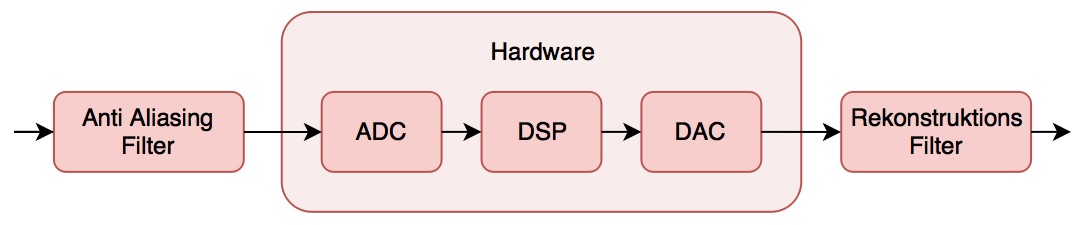
\includegraphics[width=8cm]{billeder/flow_all}
	\vspace{0.5 cm}
\end{figure}


\emph{I dette kapitel bliver der redegjort for testforløbet af equalizeren. Der bliver brugt en Bode 100 til måling af equalizerens overførselsfunktion. På denne måde kan det bevises om equalizerens profiler fungerer korrekt.}

\section{Forberedelse}


For bedst at teste equalizeren, blev der besluttet at følgende tre 3 parametre skulle gennemtestes: 

\begin{enumerate}[noitemsep,nolistsep]
    \item Amplituden/Gain
    \item Bandwidth
    \item Frekvens \\
\end{enumerate}



Under disse parametre var der en del forskellige ting der skulle tages højde for. 
\begin{enumerate}[noitemsep,nolistsep]
    \item Ved amplituden skulle der holdes en fast bandwidth ($100\hertz$) og en fast frekvens ($1\kilo\hertz$). Der blev målt hhv. $\pm5\decibel$ og $\pm7\decibel$
    \item Ved bandwidth skulle der holdes en fast amplitude ($\pm5\decibel$) samt en fast frekvens. ($1\kilo\hertz$). Her blev der målt forskellig bandwidth, hhv. $100\hertz$, $500\hertz$ og $1\kilo\hertz$.
    \item Ved frekvensen blev der holdt en fast amplitude ($\pm5\decibel$) og fast bandwidth ($100\hertz$). Her blev der dog målt med forskellige typer filtre. Peak filtret blev målt ved $100\hertz$ og $5\kilo\hertz$, hvor high shelf og low shelf filtrene blev målt ved $1\kilo\hertz$ og $5\kilo\hertz$. \\
\end{enumerate}

Derudover blev der opstillet en "kode-test" hvor der blev beregnet filtre som alle havde samme egenskaber, uanset om dette var et peak, high shelf eller et low shelf. Dette var for at eftervise om DSP koden var konsistent i alle typer filtre. \\

\section{Udførelse}
For at måle overføringsfunktionen sættes Bode 100'ens output til indgangen på equalizeren. CH1 sættes også til indgangen. CH2 sættes til udgangen og målingen foretages for samtlige af ovenstående presets. \\


\begin{figure}[h!]\label{fig:bode_setup}
	\centering
	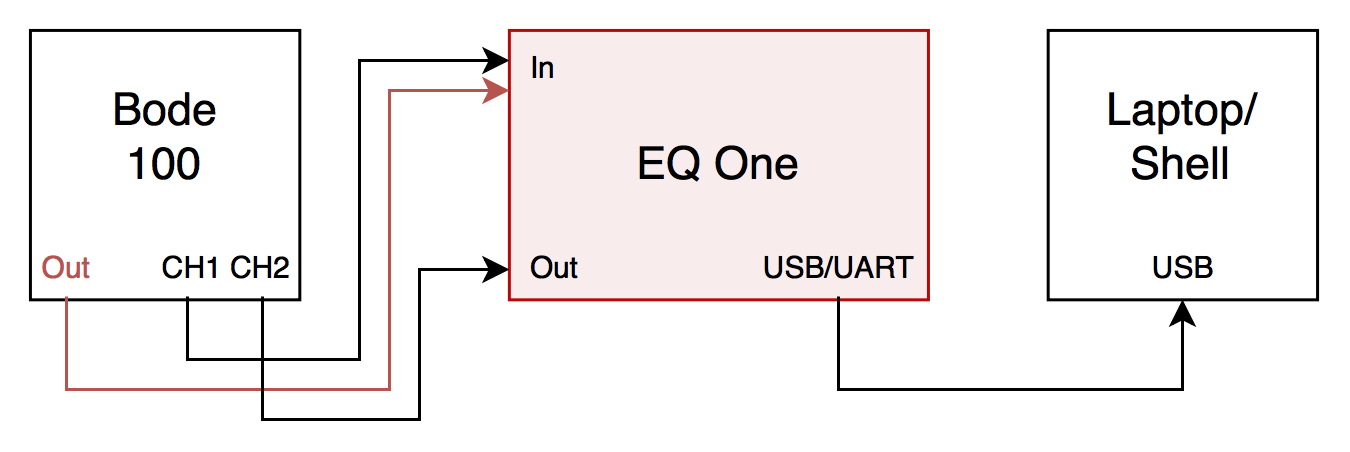
\includegraphics[width=0.7\textwidth]{billeder/bode_setup}
	\caption{Målingeopstilling af equalizer med Bode 100}
\end{figure}	

\FloatBlock

\section{Resultater}
I dette afsnit vil resultaterne af målingerne blive vist, og der vil herefter drages til delkonklusion, hvor teorien stilles op mod praktis.
Det første resultat på figur \ref{fig:eq_off1}, viser en graf hvor den digitale del er slået fra, og selve equalizeren er deaktiveret. Det er altså kun de analoge filtre der dominerer. Det teoretiske AA-filter ses til sammenligning på figur \ref{fig::afilter_aasim}. \\
Den vigtige del at eftervise, er hvor equalizeren er slået til. 
Udfra forberedelsen, skulle 3 parametre testes - amplituden, båndbredden og frekvensen. 
Da der blev målt første gang, viste det sig, at både frekvensen og amplituden afvigede med ca. en faktor 2, hvorfor der blev lavet en måling med korrigerede parametre. \\

\husk{Skal der beskrives hvad der er gjort på de korrigerede grafer?}
De teoretiske beregninger og resultater stilles op ved siden af hinanden.
Dette ses for hhv. for hvert parameter i figur: \ref{fig:gain_uden_hotfix}, \ref{fig:bandwidth_uden_hotfix} og \ref{fig:freq_uden_hotfix}. 
Her ses tydeligt den afvigende amplitude og båndbredde.

\begin{figure}[h!]
	\centering
	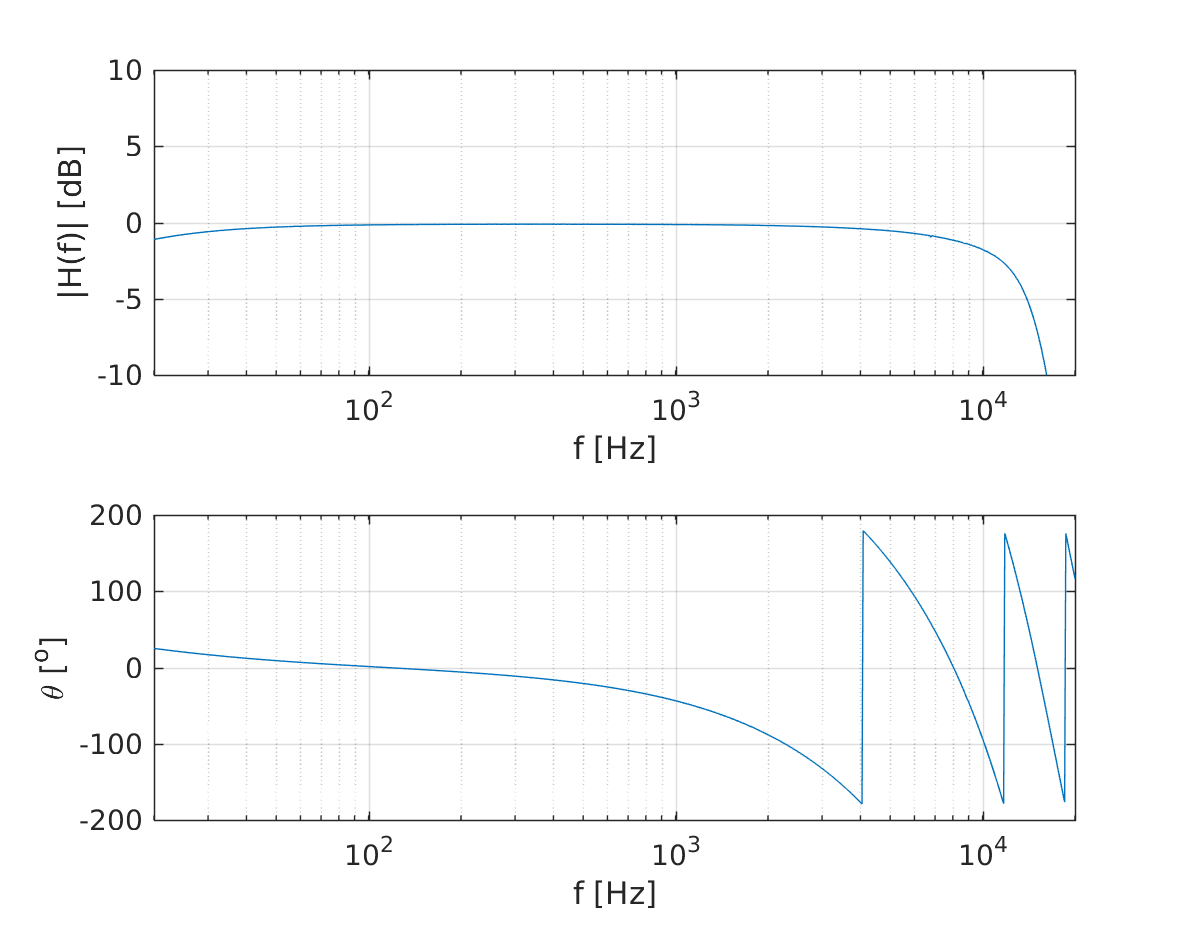
\includegraphics[scale = 0.8]{matlabdemo/test/test_eq_off.png}  
	\caption{Måling af hele systemet uden equalizer slået til.}
	\label{fig:eq_off1}
\end{figure}

\subsection{Målinger}

\begin{figure}[h!]
	\centering
	\subbottom[]{%
	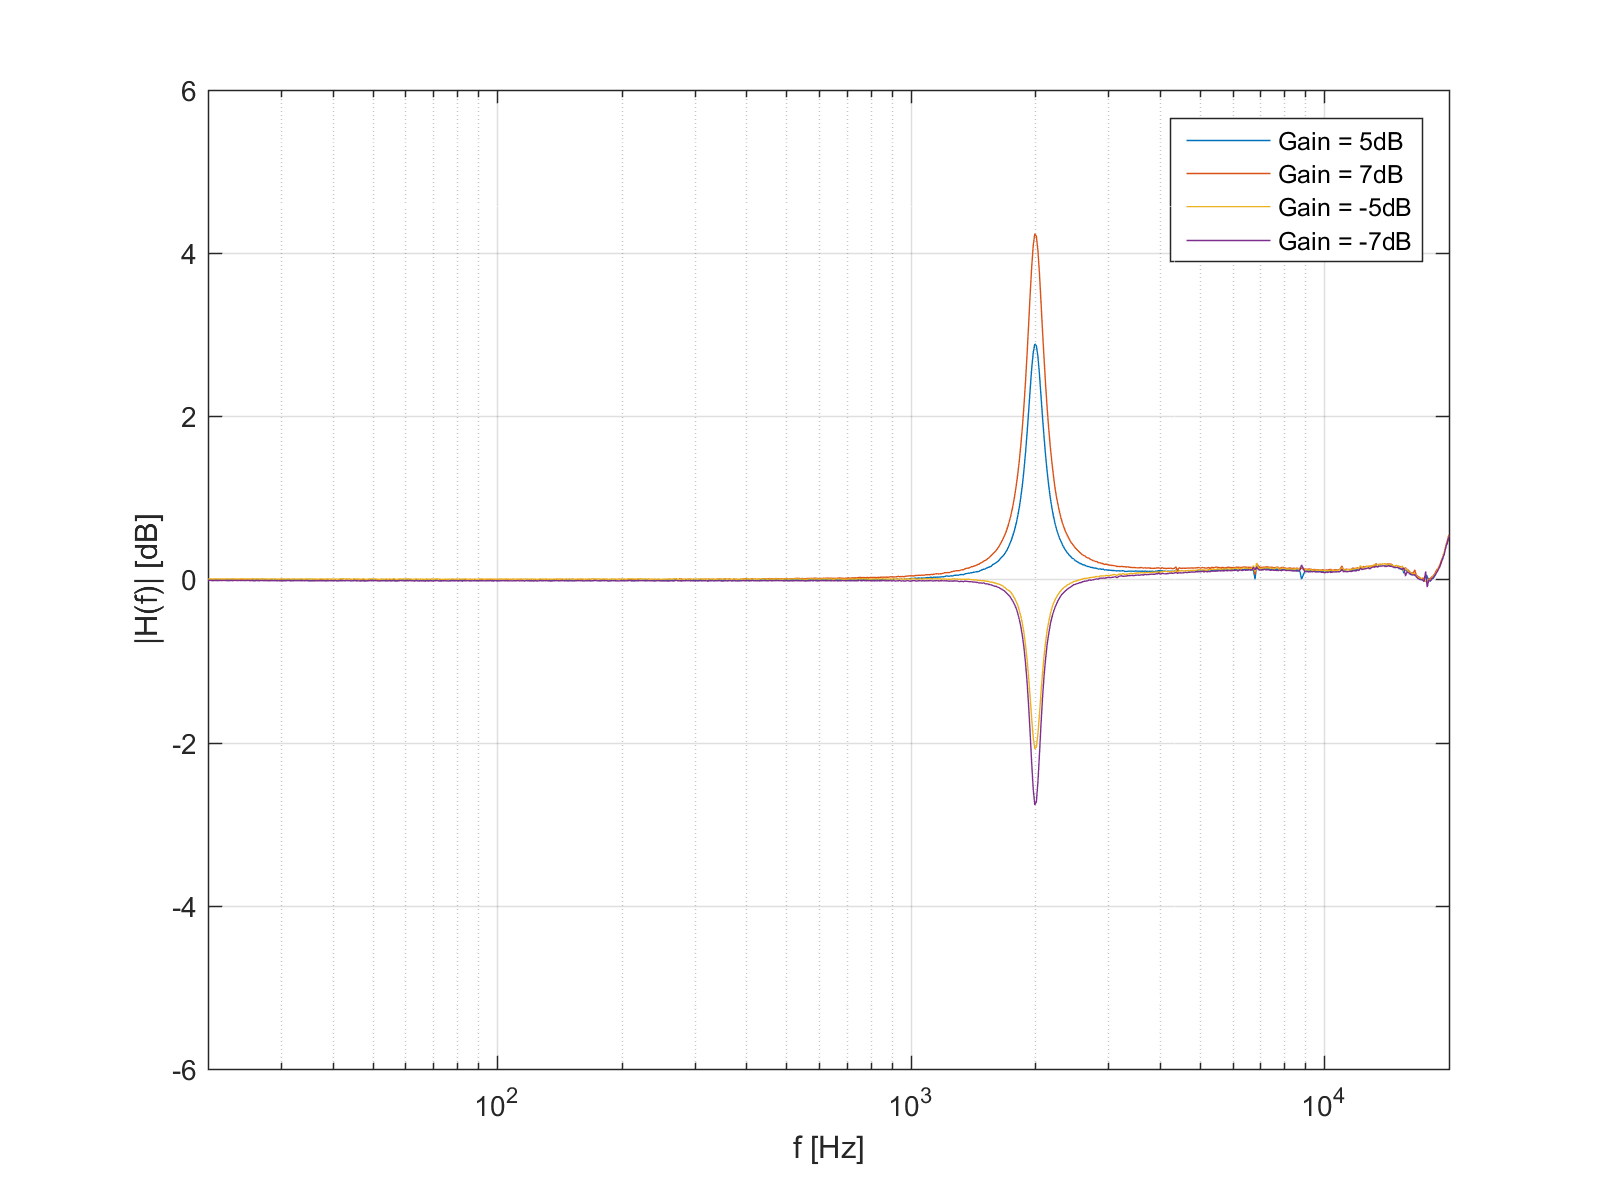
\includegraphics[width=7cm]{billeder/Gain_uden_hotfix}
	\label{fig:gain_uden_hotfix}}
	\subbottom[]{%
	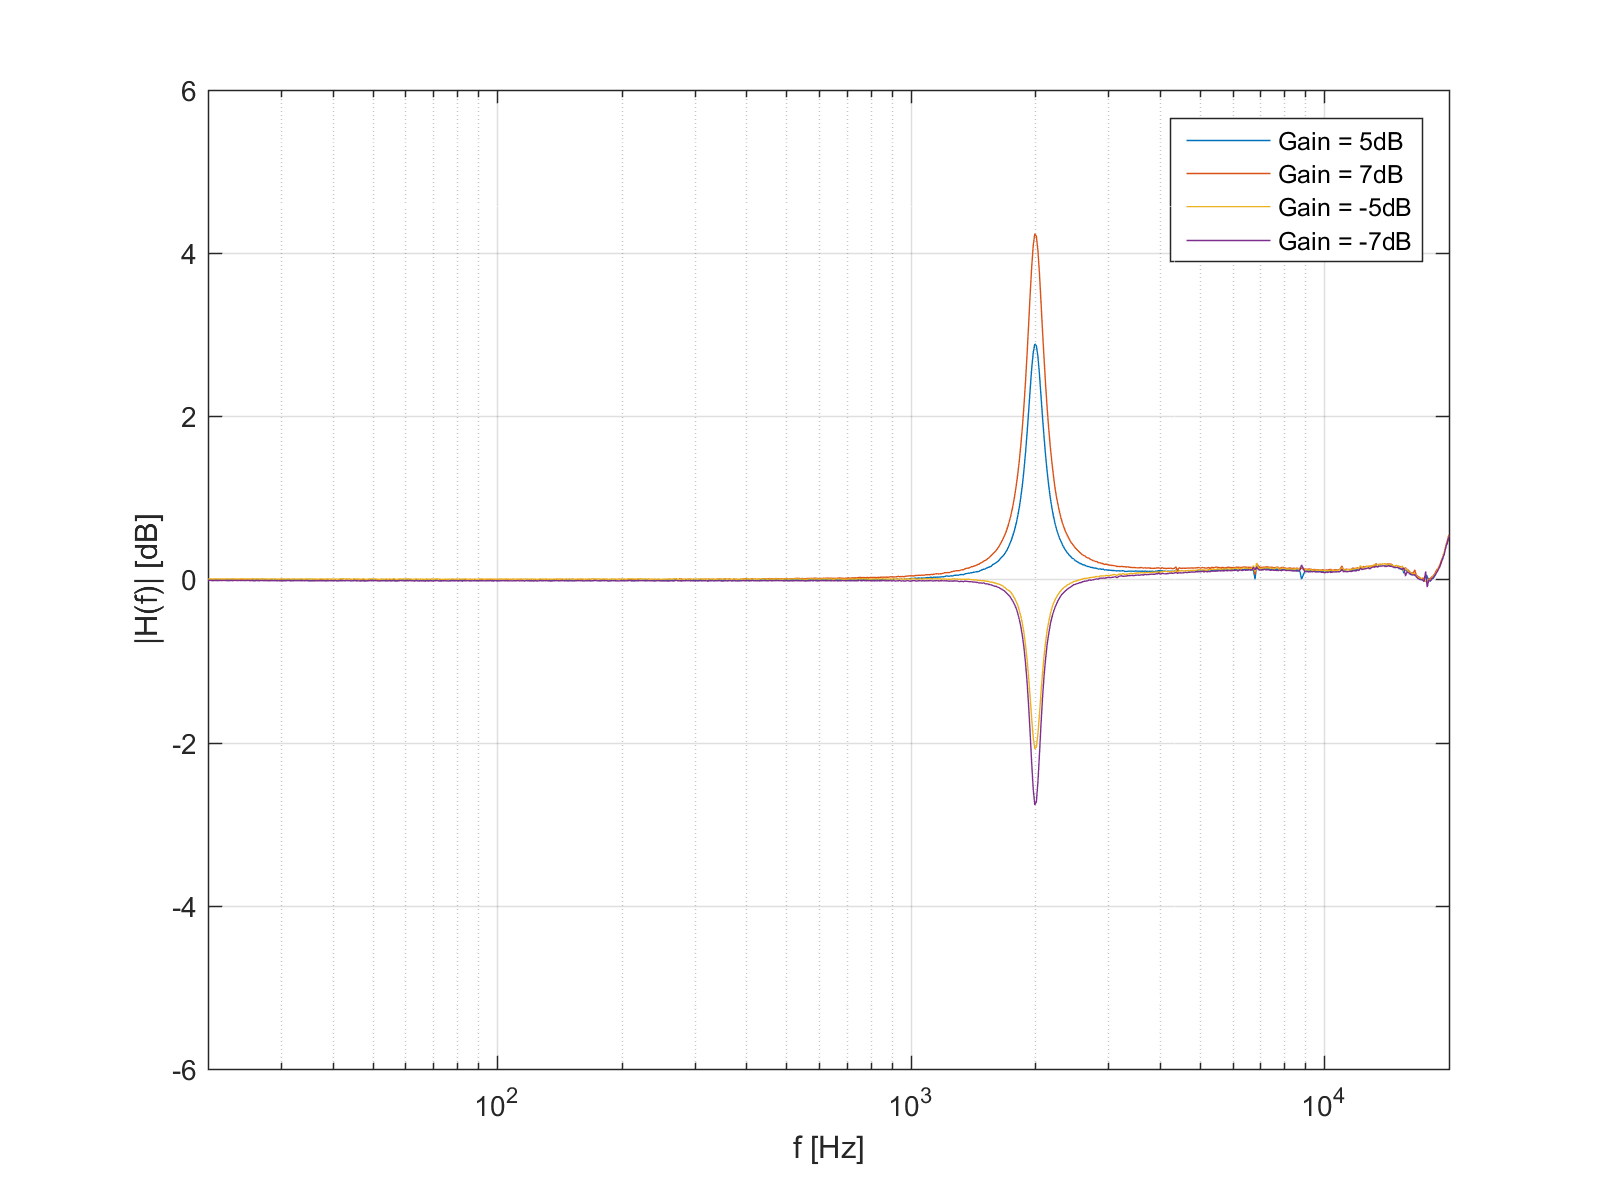
\includegraphics[width=7cm]{billeder/Gain_uden_hotfix}
	\label{fig:gain_teori}}
  	\caption{Målingsresultat af hhv. gain $5\si{\dB}$, $7\si{\dB}$, $-5\si{\dB}$ og $-7\si{\dB}$ uden korrigering}
	\label{fig:gain}
\end{figure}

\begin{figure}[h!]
	\centering
	\subbottom[]{%
	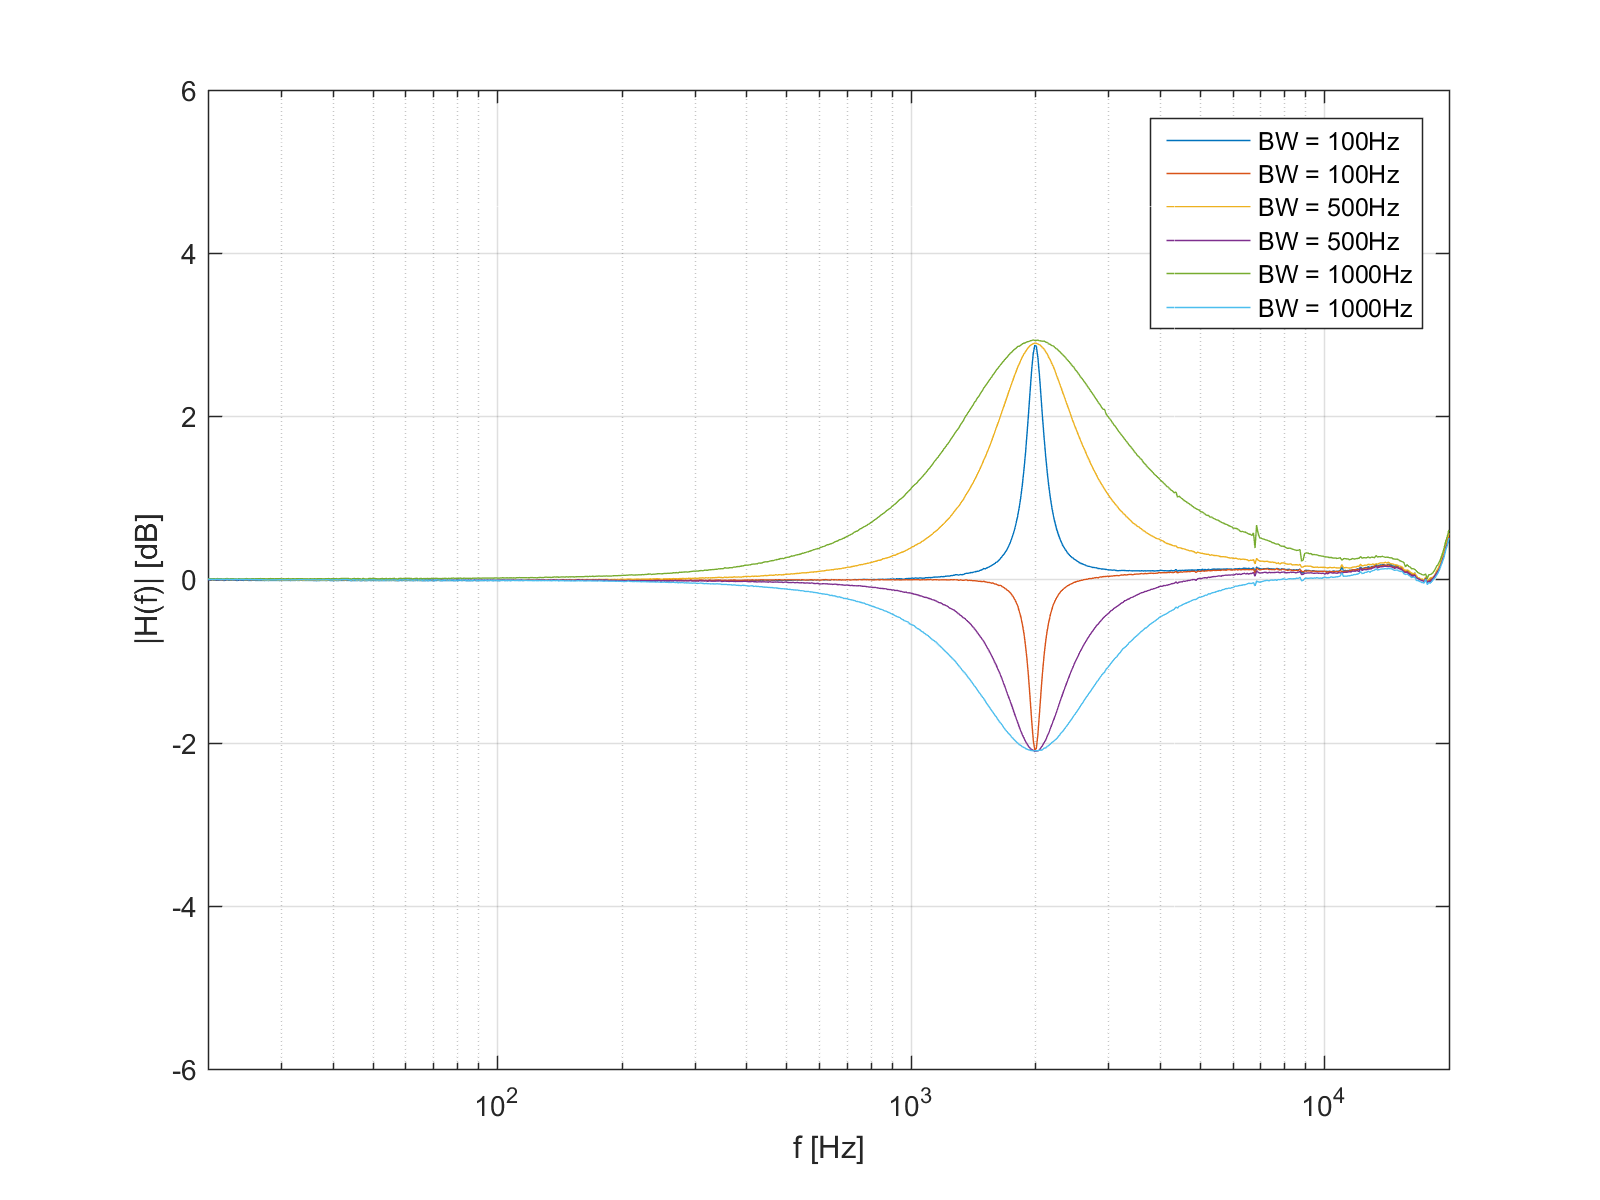
\includegraphics[width=7cm]{billeder/Bandwith_uden_hotfix}
	\label{fig:bandwidth_uden_hotfix}}
	\subbottom[]{%
	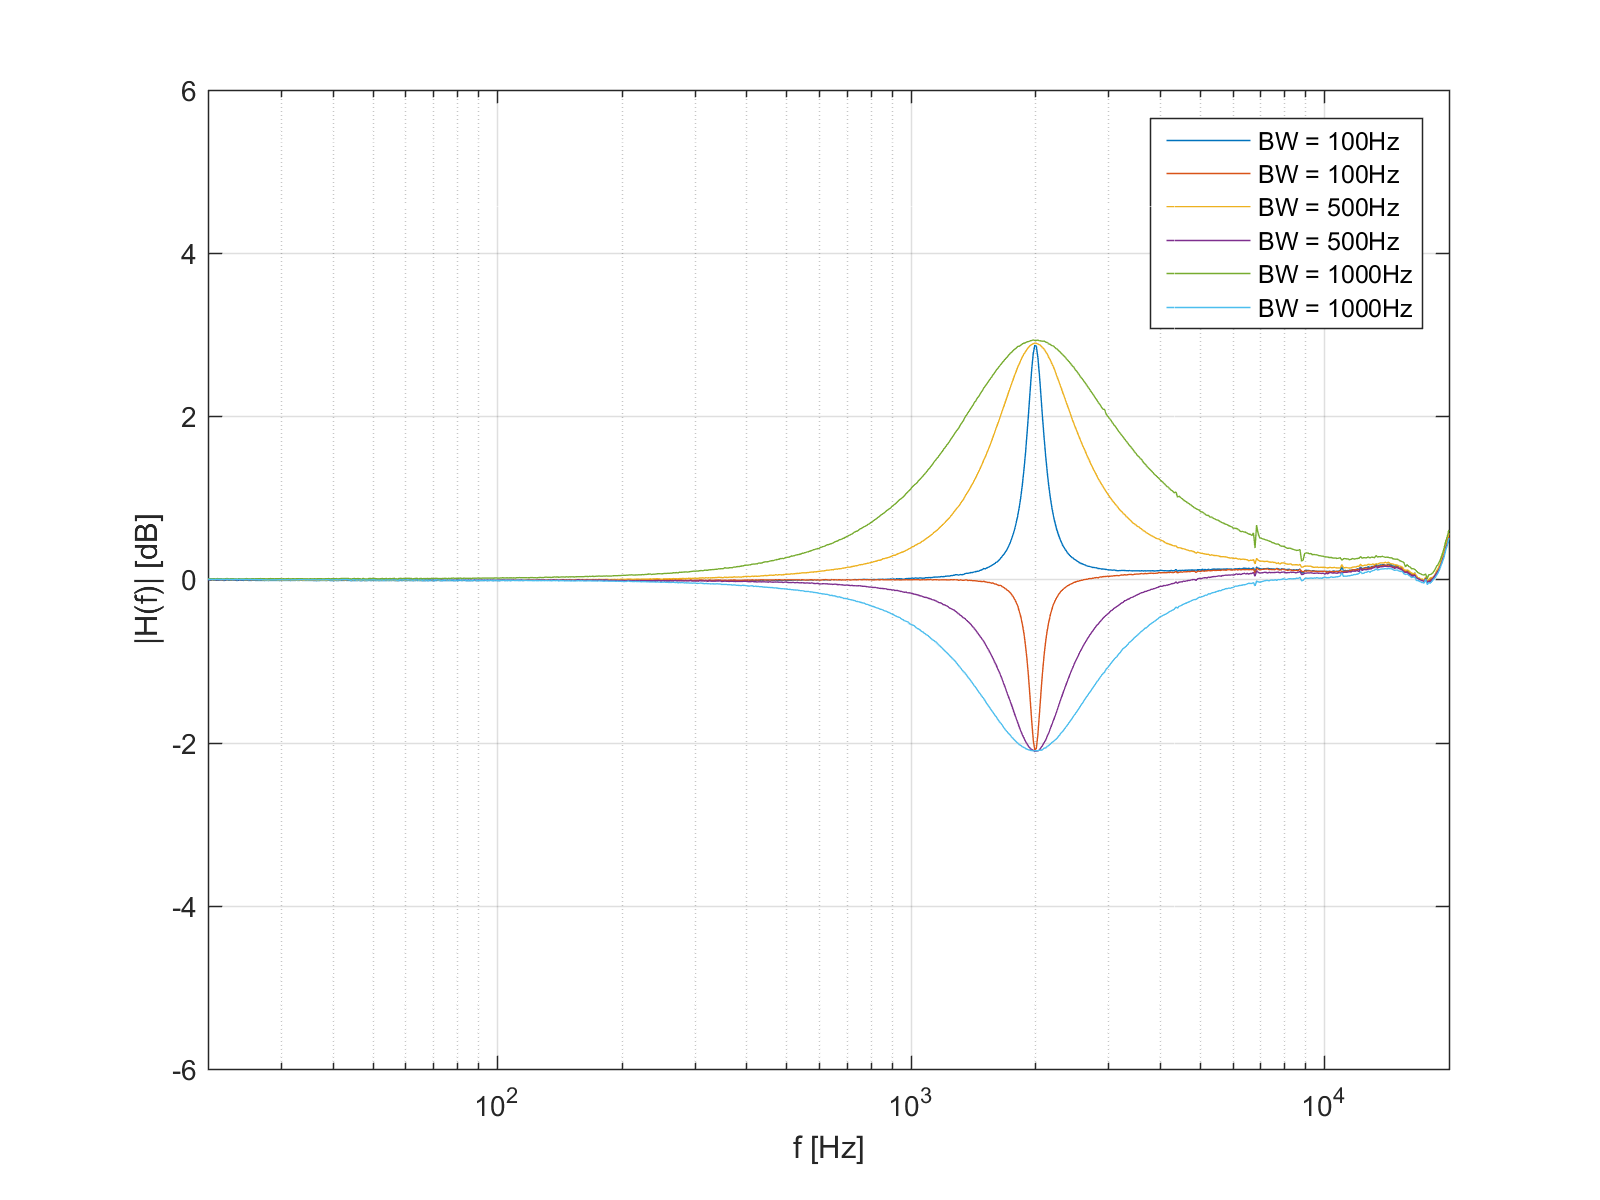
\includegraphics[width=7cm]{billeder/Bandwith_uden_hotfix}
	\label{fig:bandwidth_teori}}
  	\caption{Målingsresultat af bandwidth med hhv. 100hz, 500hz og 1000hz.}
	\label{fig:gain}
\end{figure}

\begin{figure}[h!]
	\centering
	\subbottom[]{%
	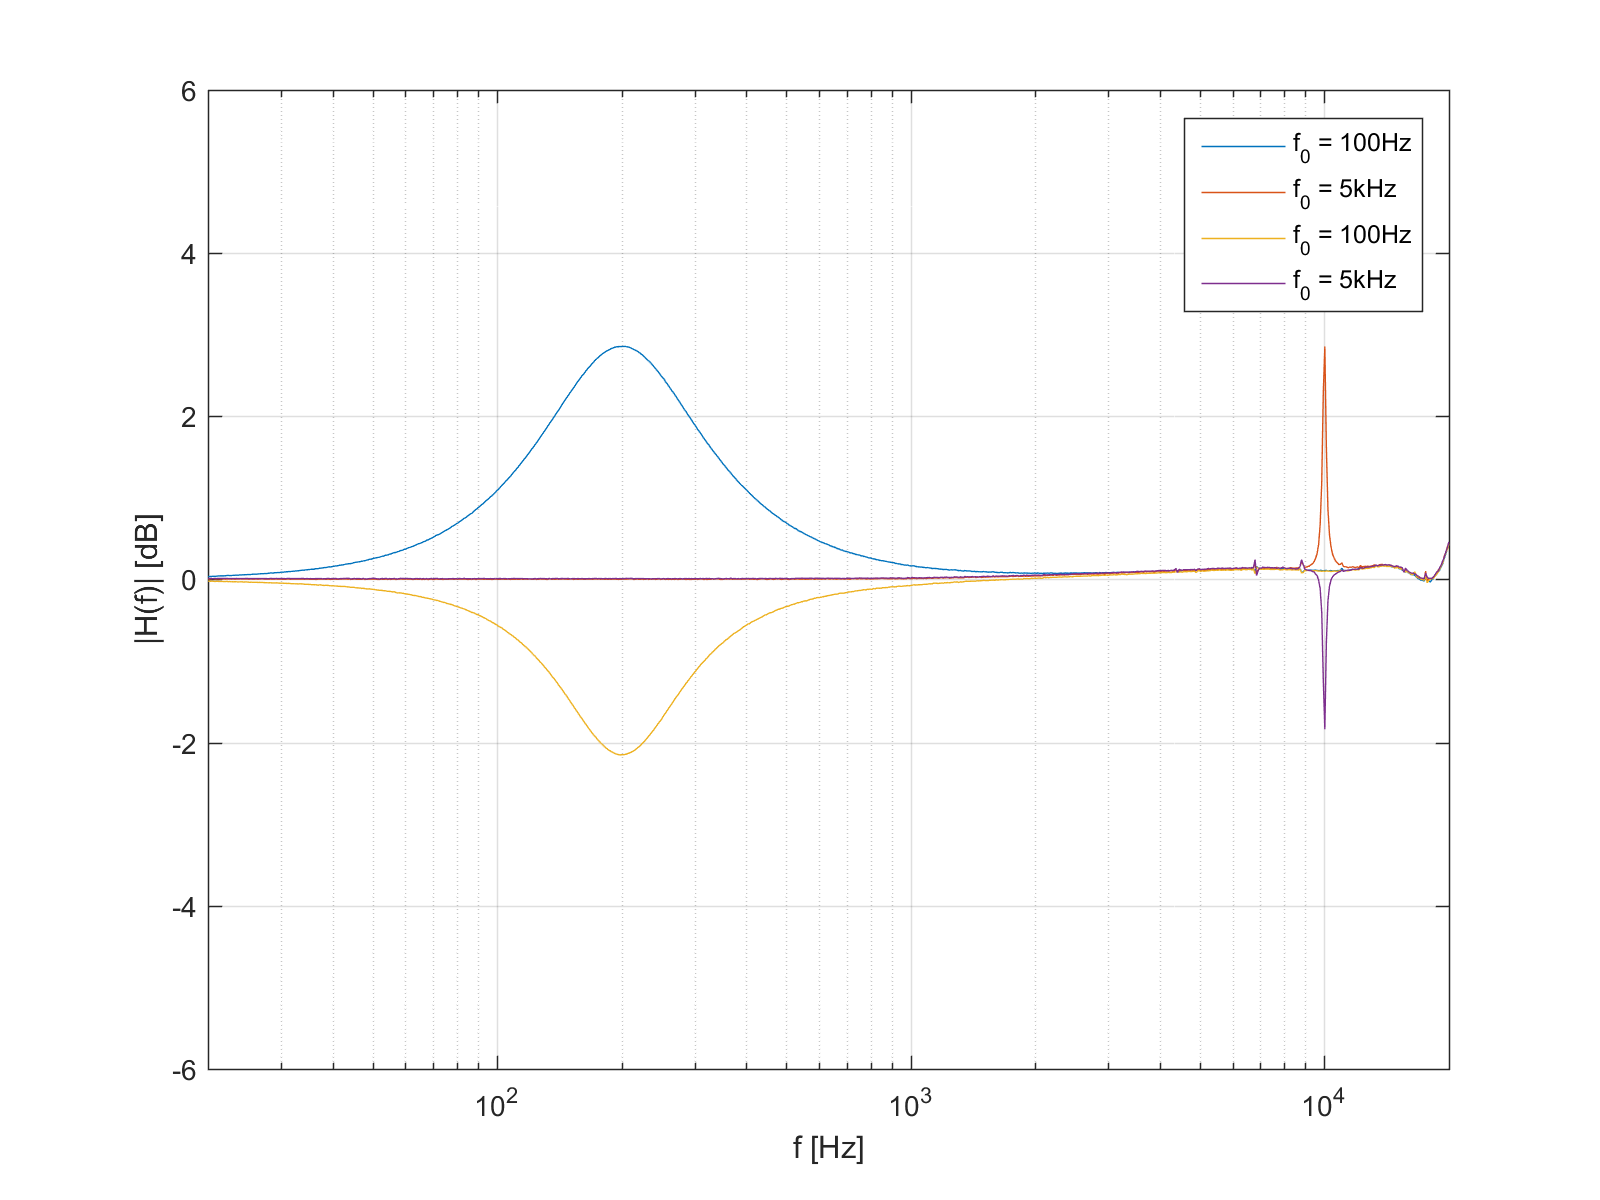
\includegraphics[width=7cm]{billeder/Frekvensplacering_uden_hotfix}
	\label{fig:freq_uden_hotfix}}
	\subbottom[]{%
	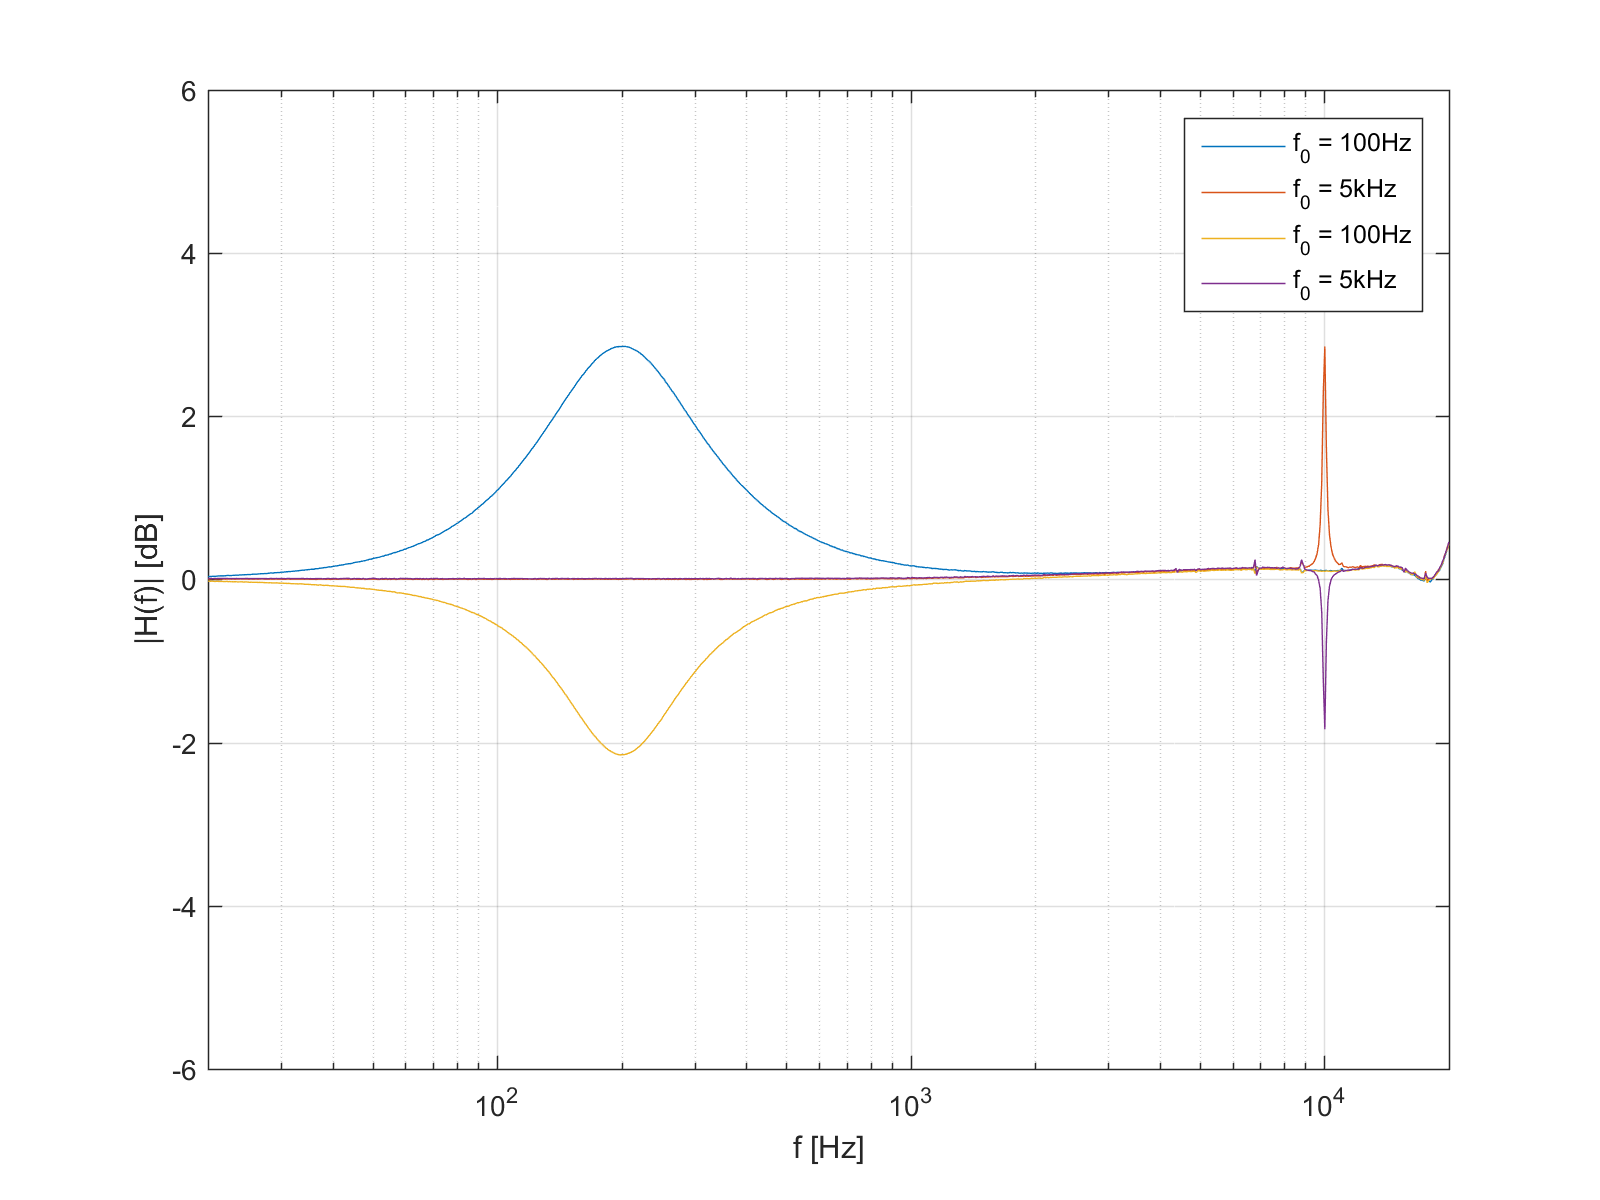
\includegraphics[width=7cm]{billeder/Frekvensplacering_uden_hotfix}
	\label{fig:freq_teori}}
  	\caption{Målingsresultat af frekvensen i hhv. 100hz og 5kHz}
	\label{fig:gain}
\end{figure}

\begin{figure}[h!]
	\centering
	\subbottom[]{%
	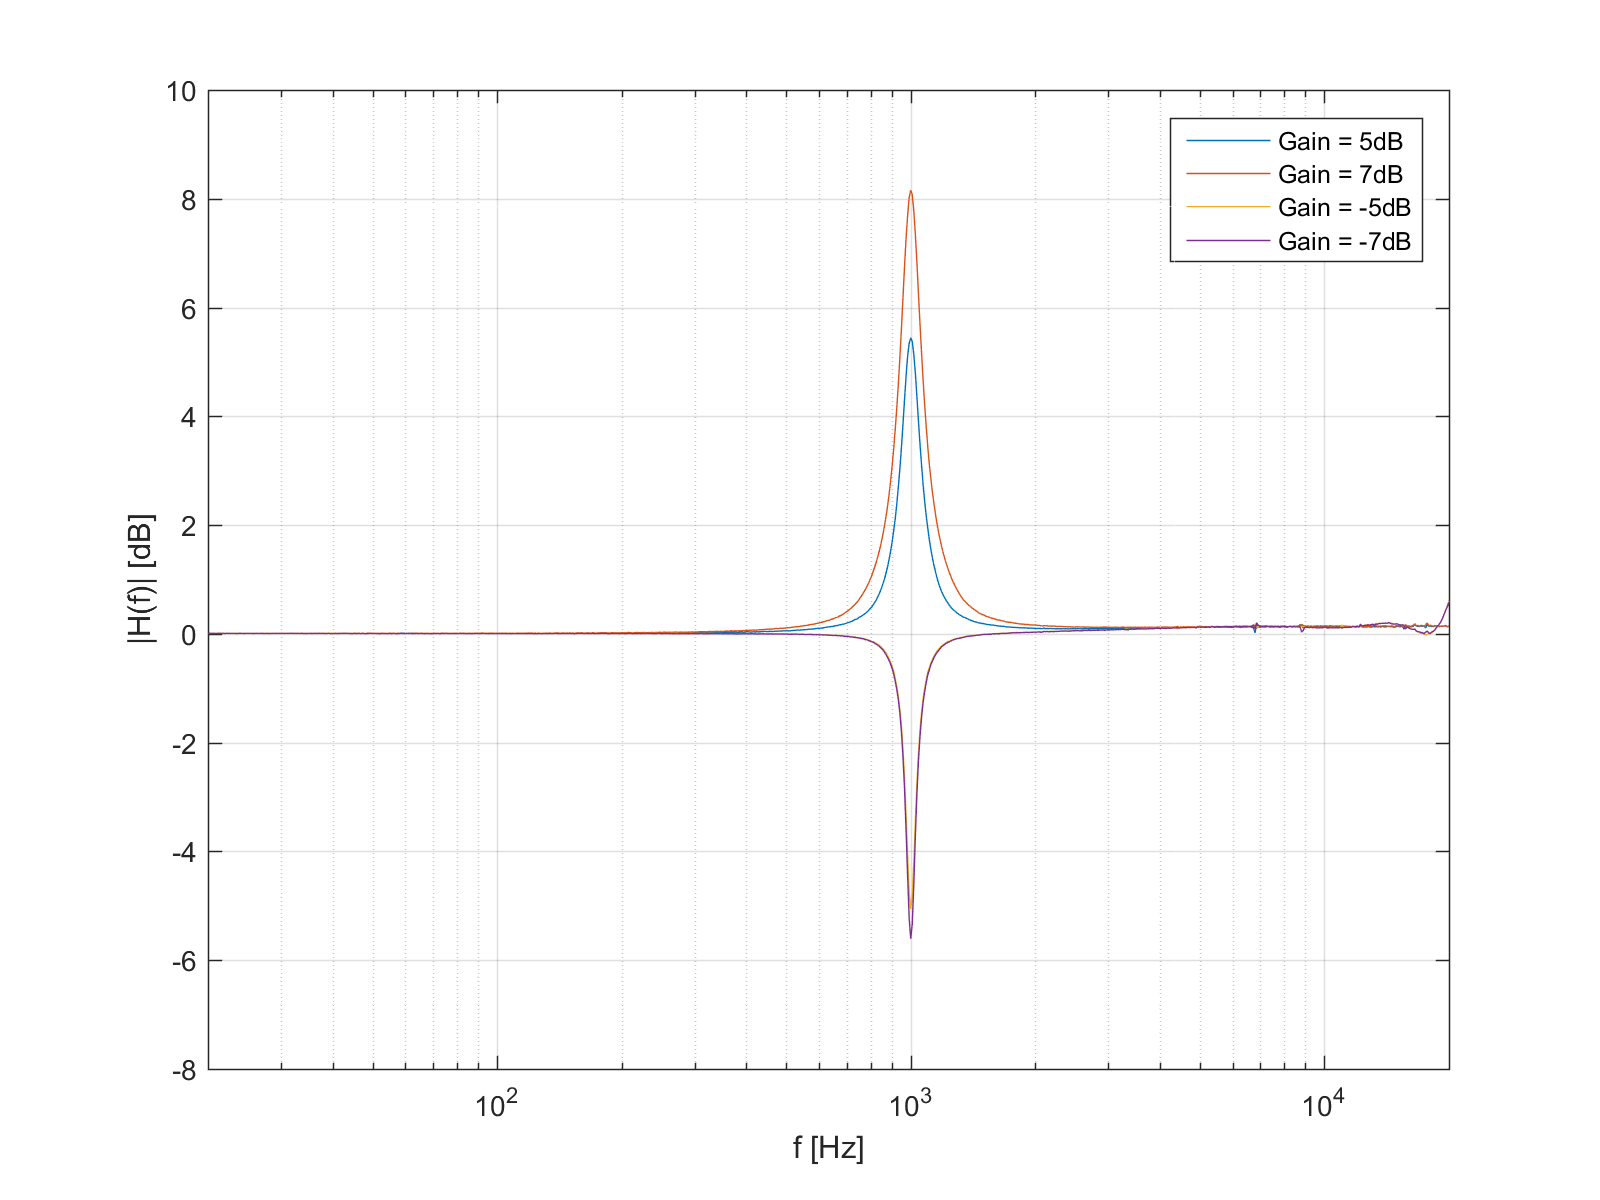
\includegraphics[width=7cm]{billeder/Gain_Med_hotfix}
	\label{fig:gain_med_hotfix}}
	\subbottom[]{%
	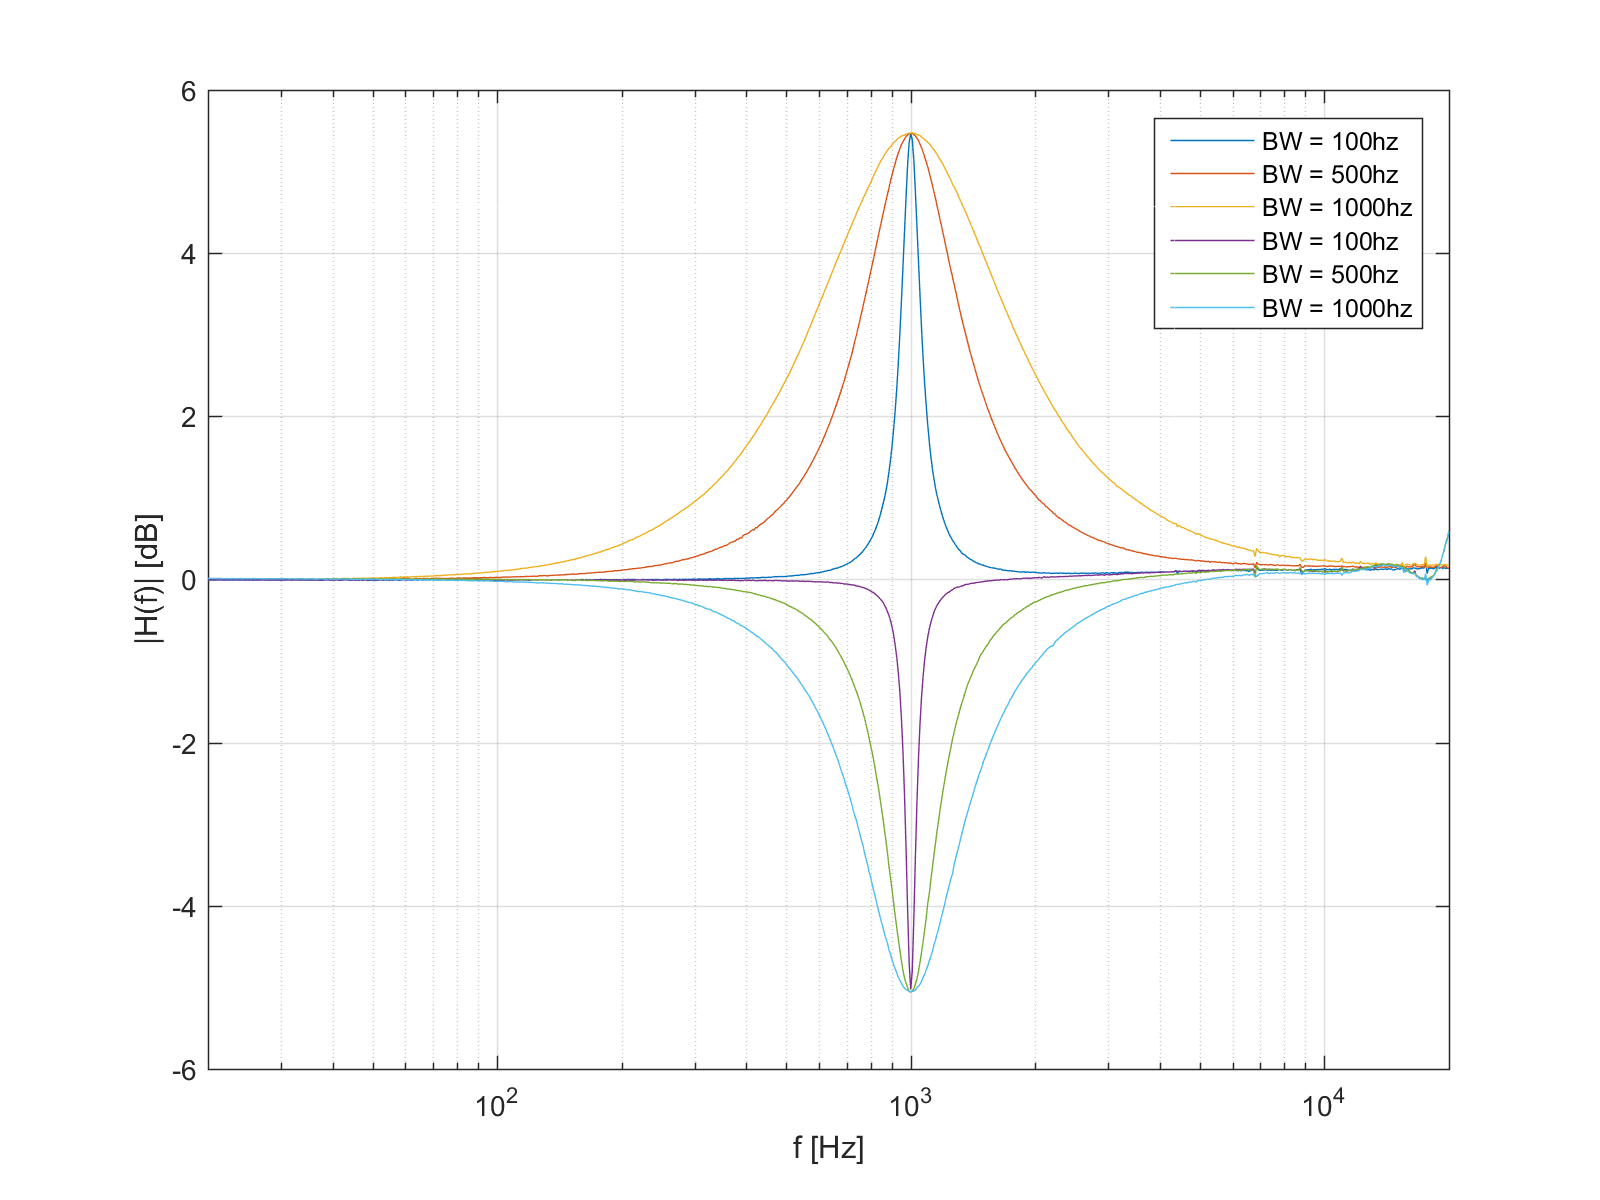
\includegraphics[width=7cm]{billeder/Bandwidth_Med_hotfix}
	\label{fig:bandwidth_med_hotfix}}
  	\caption{Her ses de korrigerede værdier}
	\label{fig:gain}
\end{figure}

\begin{figure}[h!]\label{fig:Frekvensplacering_med_hotfix}
	\centering
	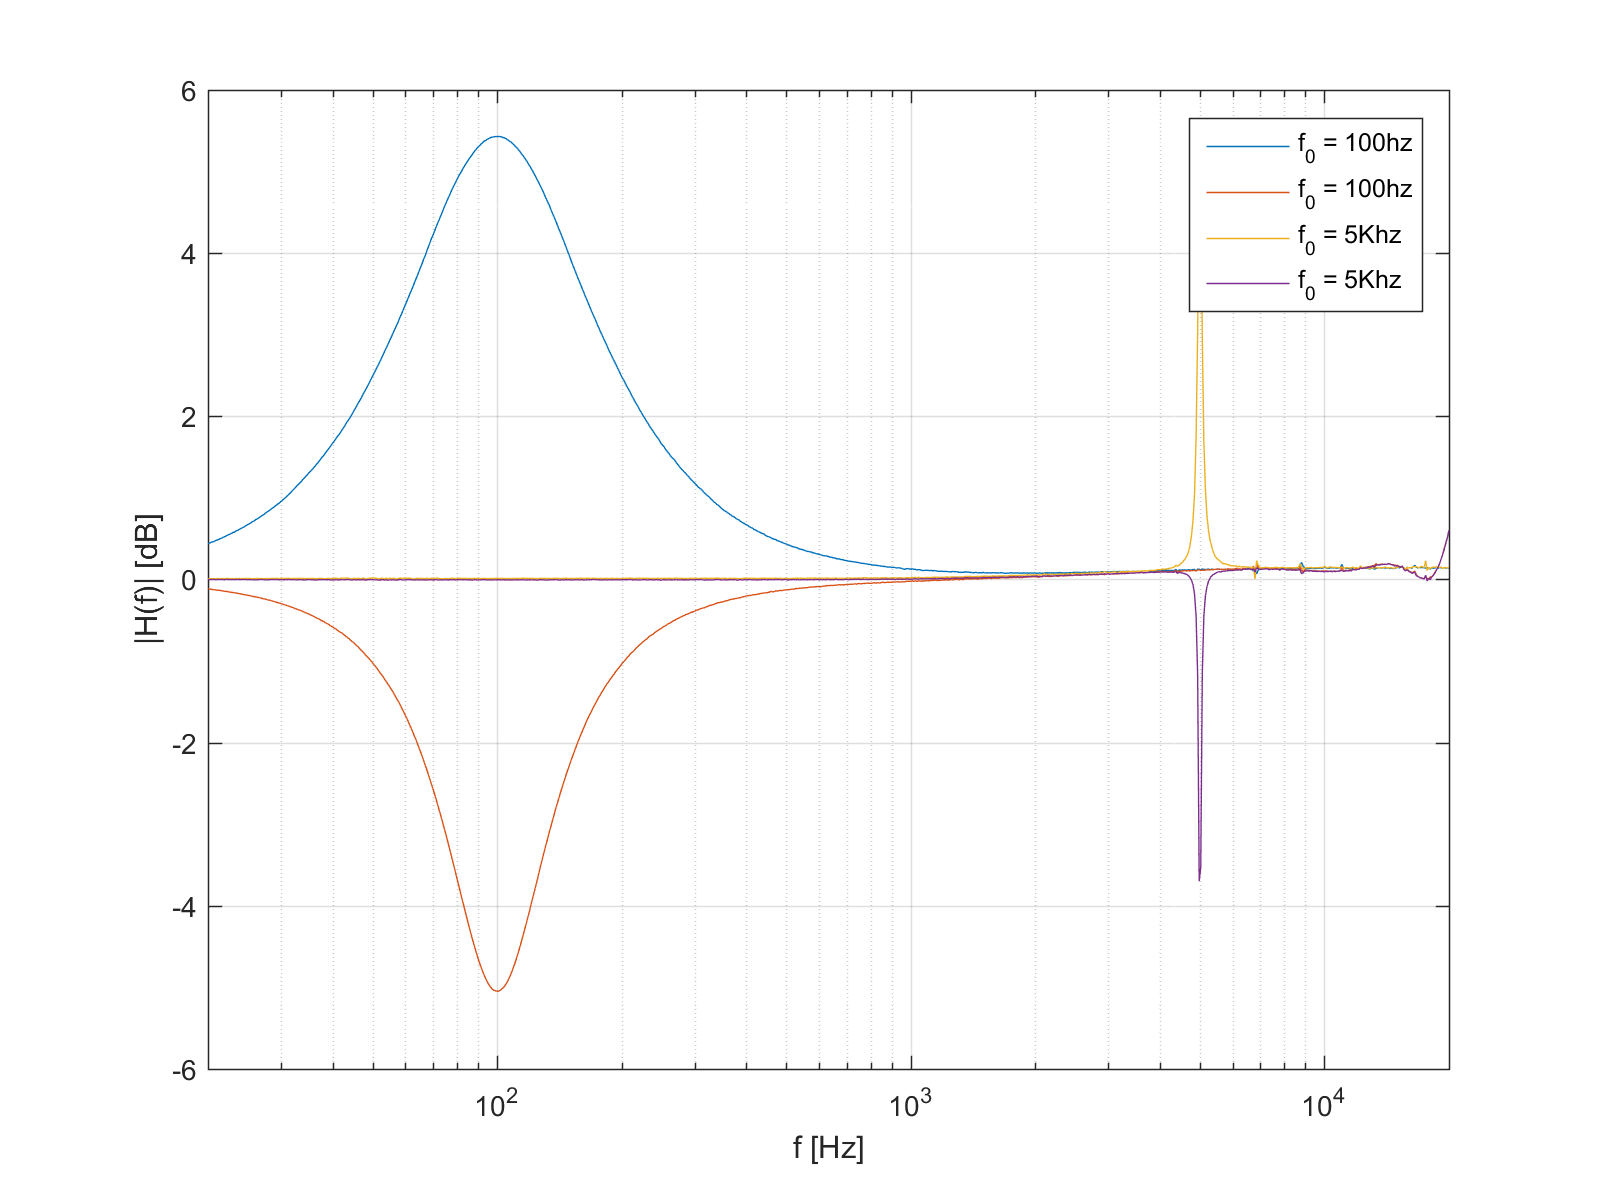
\includegraphics[width=7cm]{billeder/Frekvensplacering_Med_hotfix}
	\caption{Målingssetup med Bode 100}
\end{figure}

\section{Delkonklusion}



